\documentclass[10pt,twocolumn]{article}
\usepackage[utf8]{inputenc}
\usepackage{graphicx}
\usepackage{listings}
\usepackage{float}
\usepackage{amsmath}
\usepackage{cleveref}
\title{\textbf{CGRA optimization}}
\author{R\"{o}bke Geenen}
\date{\today}
\begin{document}
\maketitle

This report and the work discussed within are the result of a
cooperation between R\"{o}bke Geenen, Maik Vermeulen and Elbert van de
Put.

\section{Introduction}
\label{sec:introduction}
After implementing the bypass exercise from the given CGRA cookbook as
a warm-up exercise, it quickly became obvious that the given naive
implementation of the butterworth filter was indeed very naive, both
in its architecture and in the assembly implementation. Therefore it
was decided to not take the given naive implementation, nor the
implementation with the bypass exercise implemented as the starting
point, but rather redesign both the architecture and the assembly
implementation from scratch. In the following two sections, the newly
implemented architecture and the newly implemented assembly will be
discussed. Afterwards the results from the new implementation will
also be discussed shortly.


\section{Architecture}
\label{sec:architecture}
\begin{figure}[ht]
  \centering
  \caption{A schematic overview of the architecture of the improved
    implementation.}
  \label{fig:architecture}
  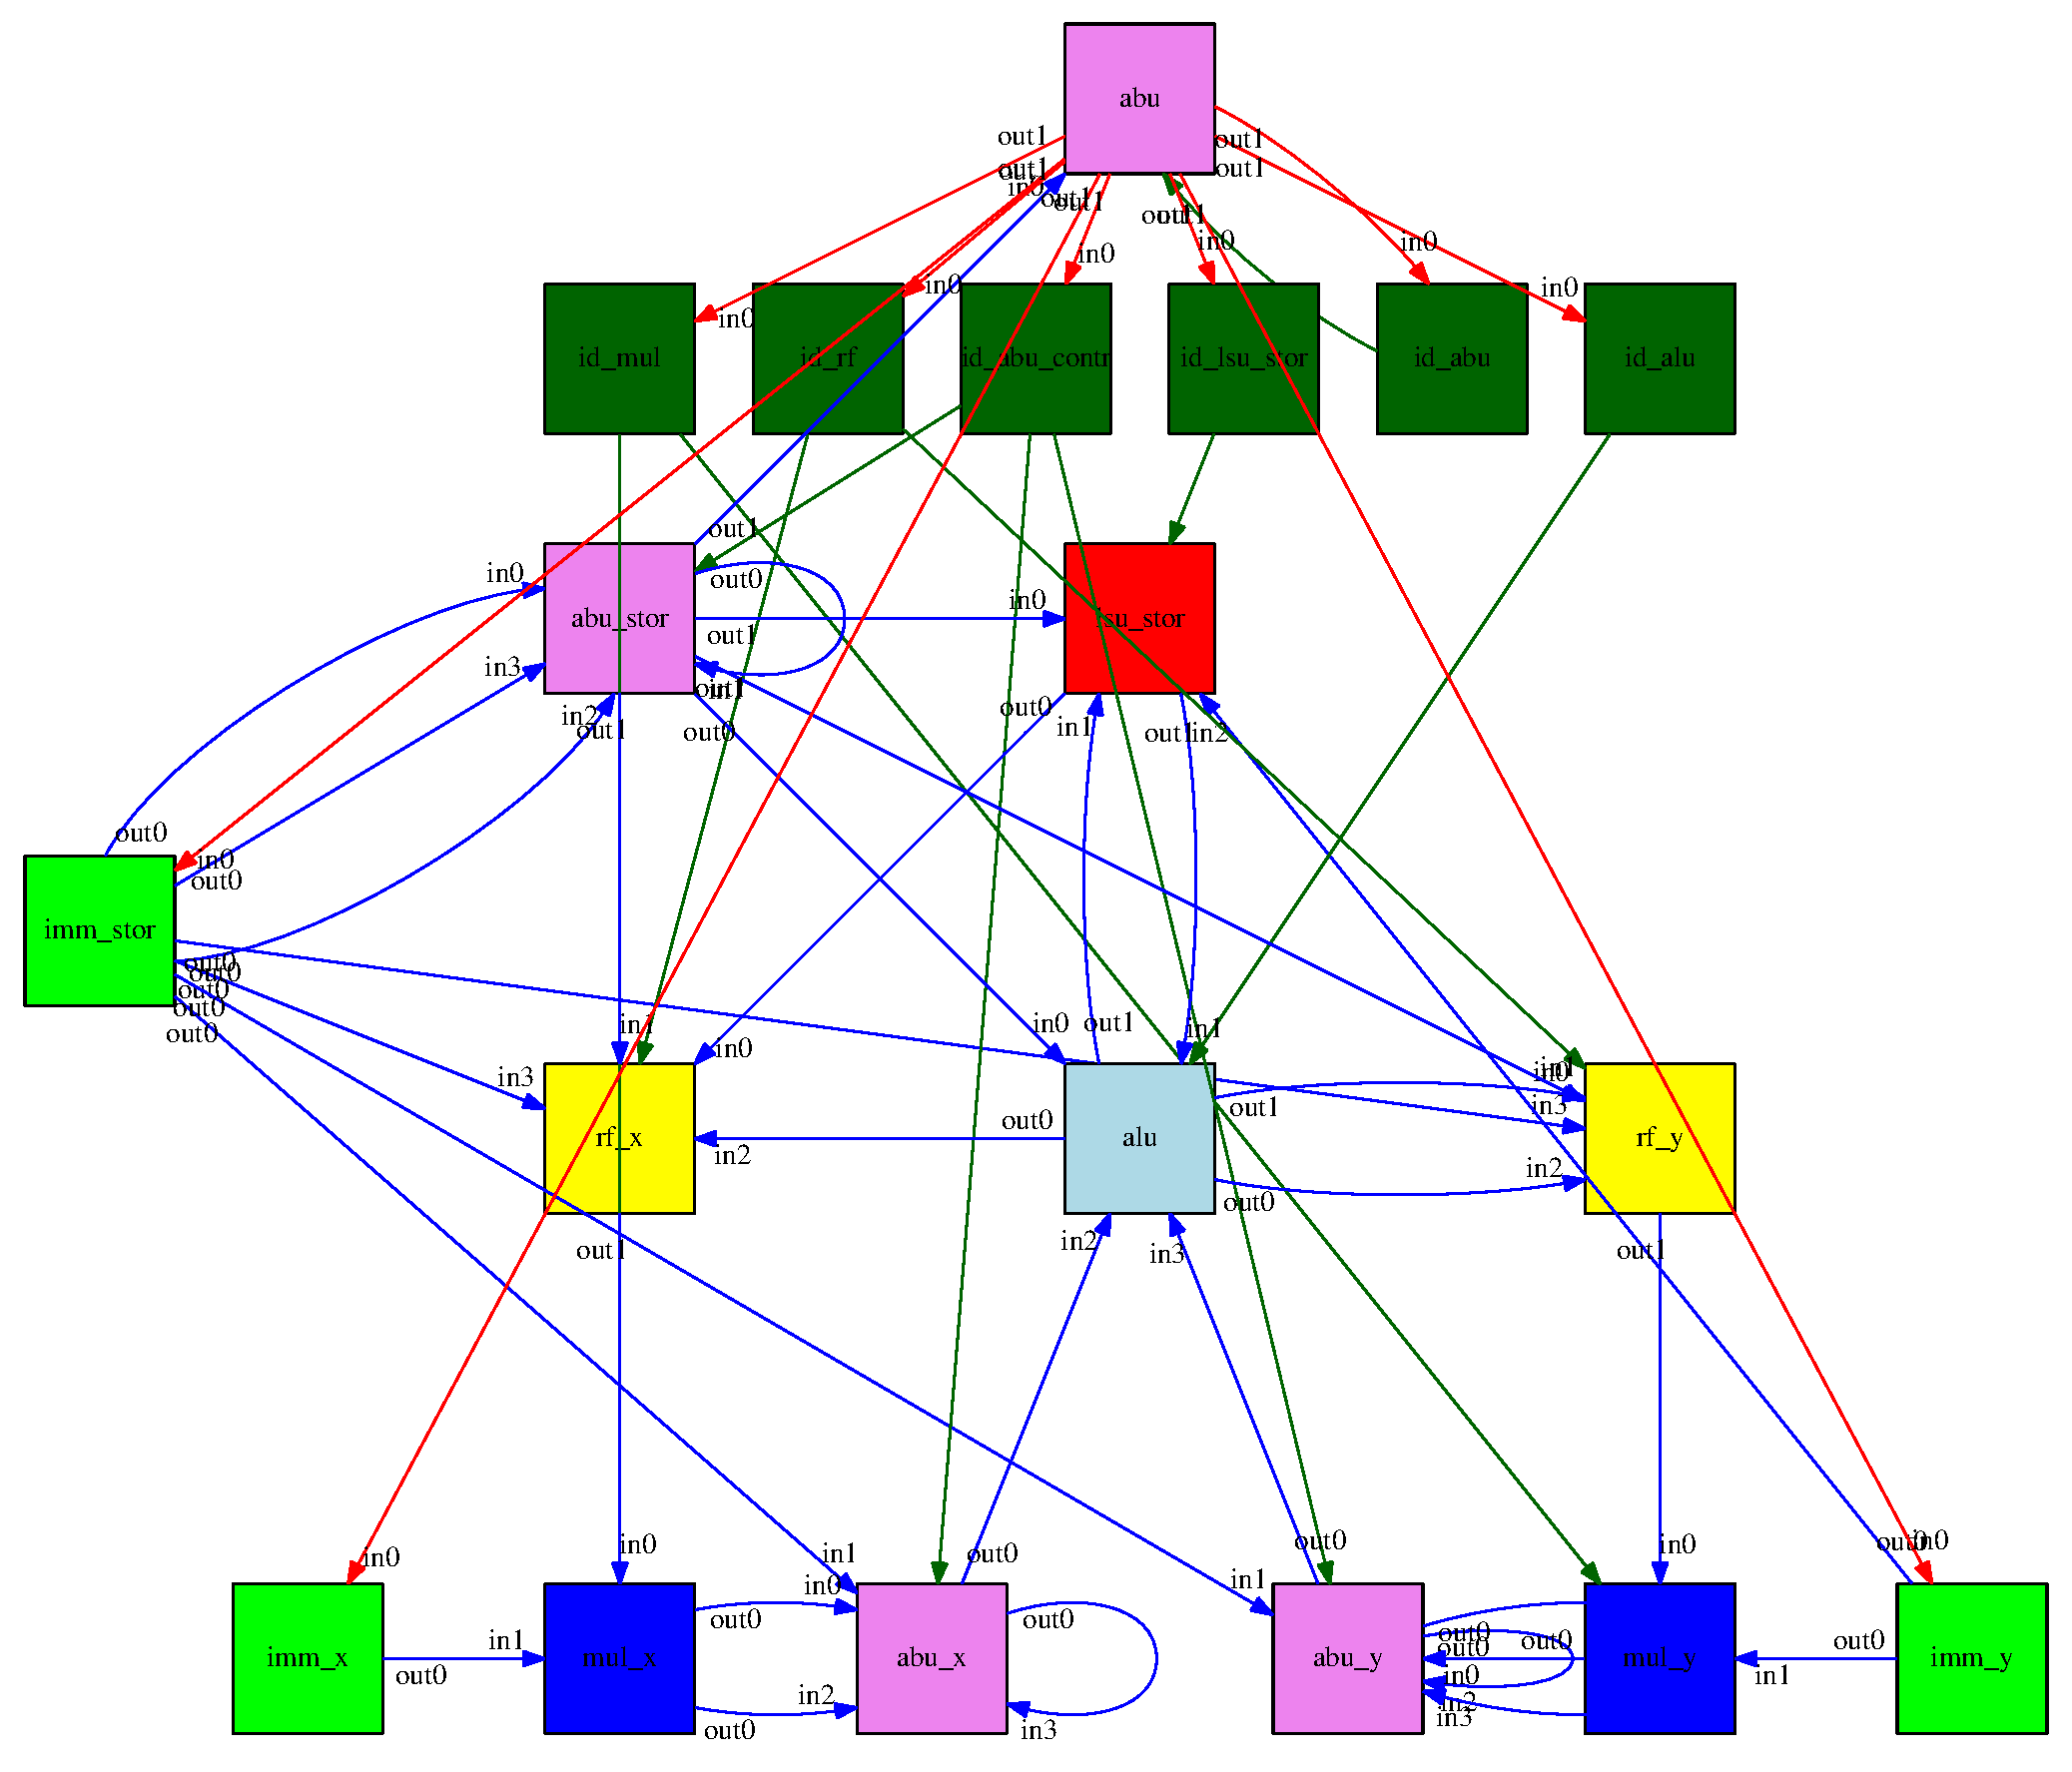
\includegraphics[width=\linewidth]{architecture.eps}
\end{figure}

All units used in the improved implementation can be seen
in~\Cref{fig:architecture}. The signal samples are stored in the
global memory of the CGRA, so a load store unit (\texttt{lsu\_stor})
is included in the architecture to be able to load input samples and
store output samples. An accumulation unit (\texttt{abu\_stor}) is
also included to store and increment the addresses of the input and
output samples. This approach is preferred over using two load store
units and using their auto address incrementing function, because the
program will have to keep track of some other small data, like a loop
counter, which will also fit in \texttt{abu\_stor}. Since a load store
unit only allows for one auto-incrementing address, two load store
units would be needed if that functionality would be desired for both
the input and the output addresses. Using only a single load store
unit also has the added benefit of eliminating any possible memory
contention, since all memory accesses will need to go through
\texttt{lsu\_stor}, so any possible memory contention will need to be
solved actively in the assembly code.

Since the butterworth filter needs to perform calculations both on
multiple past input samples as well as on multiple past output
samples, two register files (\texttt{rf\_x} and \texttt{rf\_y}) are
present in the architecture, \texttt{rf\_x} stores the last input
samples and \texttt{rf\_y} stores the last output samples. Using
register files for this means that only two memory accesses are
necessary for each sample calculated. One memory access to load the
input sample and one memory access to store the newly calculated
output sample. One register file per input and output stream suffices
as long as the order of the filter is lower than the number of
registers in the register file.

Next to the two register files, two multiplier units (\texttt{mul\_x}
and \texttt{mul\_y}) are also present in the architecture. A nice
symmetry in the filter means that it is possible to keep the two
multipliers busy at the same time. This is because for every past
sample index, both the input sample and the output sample need to be
multiplied by a certain weight, which can happen at the same time with
two multiplier units.

Furthermore two accumulation units (\texttt{abu\_x} and
\texttt{abu\_y}) are implemented to accumulate the results of the
input sample multiplications and the output sample multiplications
separately. This is done separately both to make sure that
\texttt{rf\_x}, \texttt{rf\_y}, \texttt{mul\_x} and \texttt{mul\_y} do
not have to wait for \texttt{abu\_x} and \texttt{abu\_y} and because
the accumulation of the output sample multiplications needs to be
subtracted from the input sample multiplications and this can not be
done by an accumulation unit.

In order to facilitate this subtraction, an arithmetic and logic unit
(\texttt{alu}) has also been included in the architecture. The
subtraction is however not the sole purpose of \texttt{alu}, it is
also used to wrap the register file addresses. This is useful to
implement the sliding action of the filter weights over the samples,
as will be detailed in~\Cref{sec:assembly}. Normally one would not
need \texttt{alu} for this purpose, because it would make sense if
\texttt{rf\_x} and \texttt{rf\_y} wrapped their own addresses.
Apparently however, the implementer of the CGRA thought that was a
stupid idea, and that it would be better to let the register file
output random stuff if an address higher than the number of registers
is requested.

Lastly two immediate units (\texttt{imm\_x} and \texttt{imm\_y}) are
present to provide \texttt{mul\_x} and \texttt{mul\_y} with weights at
the moment of multiplication. And a third immediate unit
(\texttt{imm\_stor}) is present to provide immediate values to
\texttt{abu\_stor}, \texttt{rf\_x}, \texttt{rf\_y}, \texttt{abu\_x}
and \texttt{abu\_y}. Apart from \texttt{abu\_stor}, they only use
\texttt{imm\_stor} to initialize their registers.


\section{Assembly}
\label{sec:assembly}
\resizebox{!}{\textheight}{
  \rotatebox{90}{
    \lstinputlisting[caption={The complete assembly source code for
      the improved implementation.},label={lst:assembly},captionpos=b,
    basicstyle=\tiny\ttfamily,linewidth=2\textwidth]{butterworth.pasm.tex}
  }
}

The complete assembly code of the improved implementation can be found
in~\Cref{lst:assembly}. The code starts with a small loop that loops
over all registers in \texttt{rf\_x} and \texttt{rf\_y} and clears
each register to zero. This is so the first samples calculated will be
calculated as if the input signal was zero until the first sample.
This is an often made choice in filter implementations. While there
could be other ways to do this, the given implementation chose this
approach and therefore the new implementation had to behave the same
way.

After clearing all registers, some initial values are loaded into
\texttt{abu\_stor}: the address of the register with the current
sample, the memory address of the first input sample, the memory
address of the first output sample and the total number of samples.
After initializing the registers, the program drops into the main
filter loop.

The main loop executes one iteration per sample, it starts with
loading the input sample from the input address currently stored in
\texttt{abu\_stor}, this sample is then stored in \texttt{rf\_x}.
Meanwhile the first register in \texttt{abu\_x} and \texttt{abu\_y} is
cleared. Then a series of multiplications start, each filter weight
gets its own cycle in which the appropriate input sample is loaded
from \texttt{rf\_x}, the appropriate output sample is loaded from
\texttt{rf\_y}, the input filter weight is output from \texttt{imm\_x}
and the output filter weight is output from \texttt{imm\_y}. In a
pipe-lined fashion, the result of the multiplication is accumulated in
\texttt{abu\_x} and \texttt{abu\_y} on the next cycle. \texttt{mul\_x}
and \texttt{mul\_y} do not have to wait for the accumulation, they
will execute the next multiplication on the next cycle. Furthermore
two is added to the current register address in \texttt{abu\_stor}.
Since the multiplications with the zero filter weights are useless,
they have been skipped. Therefore the register address is incremented
by two instead of by one.

Instead of coming directly from \texttt{abu\_stor}, the register
address first passes through \texttt{alu} where a bit-wise and is
performed on the address with a bit-mask. This causes the register
address to wrap around once it grows larger than the number of
registers in the register file. The bit-mask used for this operation
is stored in one of the auto address increment configuration registers
of \texttt{lsu\_stor}. This is possible since the auto address
incrementing function is not used. This avoids the need for yet
another immediate unit.

After all sample-weight combinations have been multiplied and
accumulated, the sub-results are passed from \texttt{abu\_x} and
\texttt{abu\_y} to \texttt{alu} where \texttt{abu\_y} is subtracted
from \texttt{abu\_x}. The register address of the current sample in
\texttt{abu\_stor} is incremented by the number of registers minus the
order of the filter. This causes the register address to wrap back to
the register address of the current sample. The result of \texttt{alu}
is then stored in \texttt{rf\_y} on the register address in
\texttt{abu\_stor} and on the output memory address currently in
\texttt{abu\_stor}. Next the register address of the current sample in
\texttt{abu\_stor} is decremented by one, which causes the next
iteration of the main loop to calculate the weights over the shifted
samples. This avoids the need to manually move all the samples in the
register file by one.

Lastly the input and output memory addresses stored in
\texttt{abu\_stor} are incremented by four bytes, or one word, to
point to the next sample in memory. Also the number of samples in
\texttt{abu\_stor} is decremented by one. If the number of samples is
not zero, the branch back to the start of the main loop is taken. If
the number of samples is zero, then all samples have been calculated
and stored, the branch is not taken and the final jump to zero is
taken, which halts the execution of the CGRA.


\section{Results}
\label{sec:results}
\begin{table}
  \centering
  \caption{Different metrics for the naive implementation and the
    improved implementation.}
  \label{tbl:results}
  \resizebox{\linewidth}{!}{
    \begin{tabular}{|l||r|r||r|}
      \hline
      Metric             & \texttt{naive}        & \texttt{rbtr1}        & Improvement ($\%$) \\ \hline\hline
      Energy ($pJ$)      & $8813057.25$          & $1375805.5$           & $15.61$            \\ \hline
      Delay ($Cycles$)   & $896146$              & $38072$               & $4.25$             \\ \hline
      Area ($um^{2}$)    & $89819.0$             & $183397.0$            & $204.19$           \\ \hline
      EDAP               & $7.09371\cdot10^{17}$ & $9.60627\cdot10^{15}$ & $1.35$             \\ \hline
      SLOC               & $162$                 & $30$                  & $18.52$            \\ \hline
      Number of FUs      & $6$                   & $12$                  & $200.00$           \\ \hline
      Code size          & $972$                 & $360$                 & $37.04$            \\ \hline
    \end{tabular}
  }
\end{table}

Listed in~\Cref{tbl:results} are the relevant metrics for both the
given naive implementation, \texttt{naive}, and for the improved
implementation, \texttt{rbtr1}. It can be seen that the new
implementation uses only $15.61\%$ of the energy that the naive
implementation uses and it only takes $4.25\%$ of the cycles that the
naive implementation takes. These two huge improvements do not come
completely for free however. The improved implementation does take
$204.19\%$ of the silicon area of the naive implementation. This cost
in area is completely overshadowed by the improvements in speed and
energy. Looking at the multiplication of the energy, the delay and the
area (the Energy Delay Area Product or EDAP), it can be seen that the
new implementation still only has $1.35\%$ of the total cost of the
naive implementation.

A separate metric that was taken into consideration when the large
size of the original assembly file was discovered is the number of
Single Lines Of Code (SLOC) of the assembly program. It can be seen
from~\Cref{tbl:results} that the new implementation only has $18.52\%$
as much lines of code as the naive implementation has, $30$ lines
instead of $162$. Practically this means that the new implementation
would be much more maintainable, which is an important aspect for
production code. It must however be taken into consideration that each
line of code is twice as long in terms of operations per line, since
the new implementation has twice as many Function Units (FUs).
Therefore the effective code size of the new implementation is still
$37.04\%$ of the naive implementation code size.


\section{Conclusion}
Effectively the improved implementation provides an immense
improvement over the given naive implementation of more than $73$
times less cost in terms of the Energy Delay Area Product metric, with
the additional benefit that the assembly code size has shrunk
considerably.

An improvement which can be considered is to try to remove
\texttt{alu}, this will decrease both the energy consumption and the
on-die area, possibly with no or a very small penalty to the cycle
count. This would however mean that the implementation of the register
file in the CGRA will need to start wrapping its addresses.
Additionally, instead of using \texttt{alu} for the subtraction,
\texttt{mul\_x} could be used to multiply the result of
\texttt{abu\_y} with $-1$. The result of this multiplication can then
be accumulated in \texttt{abu\_x}. In that case \texttt{abu\_x} will
provide the final result instead of \texttt{alu}.


\end{document}
